%% main.tex -- HUMANE-LLM @ IUI 2027 short paper (target 8-9 pp incl. references; limit 5-9).
%% Template: CEURART single column (ceurart.cls from https://ceur-ws.org/Vol-XXX/CEURART.zip).
%% Conventions: one sentence per line. Any line whose truth depends on a number that is not
%% final ends in "%CHECK". List them with: grep -n '%CHECK' main.tex
%% Numbers come from results_macros.tex (generated) via \num{\RES{key}}.
%%
%% !! CEUR GenAI policy (https://ceur-ws.org/GenAI/Policy.html): "Using GenAI to generate new
%% !! text, such as paragraphs, or even entire sections of a paper is ethically unacceptable."
%% !! This draft contains AI-generated text. The human authors must rewrite it in their
%% !! own words, and the Declaration on Generative AI at the end must describe that use truthfully.
\documentclass{ceurart}
\sloppy

\usepackage{siunitx}
\sisetup{group-minimum-digits=4, group-separator={,}}

%% ---------- results macros ----------
\makeatletter
\newif\ifresultsfinal
\newcommand{\resdef}[2]{\expandafter\def\csname RES@#1\endcsname{#2}}
\newcommand{\RES}[1]{\ifcsname RES@#1\endcsname\csname RES@#1\endcsname\else\RESmissing{#1}\fi}
\newcommand{\RESmissing}[1]{\text{\textcolor{red}{\textbf{\texttt{[\detokenize{#1}]}}}}}
\makeatother
% results_macros.tex -- STUB. The analysis pipeline overwrites this file. Do not edit numbers by hand.
%
% Contract for the generator:
%   1. Emit \resultsfinaltrue as the first command once every key used in main.tex is defined.
%      Then siunitx parses and formats numbers. While the file is false, \num prints its
%      argument verbatim, and undefined keys show as red [key] tags.
%   2. Emit one \resdef{<key>}{<plain number>} per key. Use digits, "." and "-" only.
%      No "%" and no thousands separators; siunitx adds those.
%   3. Percentages are on a 0-100 scale. Differences are in percentage points.
%      Each interval key has the suffix _lo/_hi: a 95% family-cluster bootstrap percentile
%      interval for S2/S3 estimates and a Wilson interval for S1, as stated in main.tex.
%   4. Write a header comment that records the run id, the analysis code sha and the labels
%      used (judge final / arbiter / human), so every number traces to claims_ledger.md.
%
% Key registry (description -> source). Endpoints are pooled over 4 models unless named,
% with prompt P0 unless named.
% --- S1 (AACText; analysis/s1) ---
%  s1_n_messages            nonempty AACText messages (sent_{train,dev,test}_aac)
%  s1_loss_any(_lo,_hi)     % messages losing >=1 detected cue, POS-cap4, all dimensions
%  s1_loss_excl_agent(_lo,_hi)  same, excluding pronoun-agent loss (D-010 headline)
%  s1_loss_excl_agent_time  same, excluding agent and time
%  s1_loss_polarity         % messages whose negation cue is lost
%  s1_loss_speech_act       % messages whose speech-act cue is lost
%  s1_collision             % messages whose keyword string collides with a differently labeled source
%  s1_restore_two           % messages whose detected values are restored by <=2 chips
%  s1_inexpressible         % messages with losses the chip vocabulary cannot express
% --- S2 design counts ---
%  n_families_scored        test families in scored dimensions (expected 50)
%  n_outputs_judged         unique output texts judged
% --- Assumption / default asymmetry (bare channel) ---
%  bare_affirm_rate(_lo,_hi)  % definite bare polarity outputs that are affirmative (all prompts)
%  bare_affirm_n, bare_affirm_den   counts behind bare_affirm_rate
%  bare_commit_rate(_lo,_hi)  % bare outputs (all scored dims) committing to a definite critical value
%  bare_neg_offered_p2      % P2 polarity sets containing a negated suggestion
%  bare_speaker_rate        % bare agent-family outputs with a speaker agent
%  bare_plain_cert_rate     % bare certainty-family outputs that are plain assertions
%  bare_please_added        % bare/noncrit outputs adding please or a softener (P0)
%  action_gap_polarity(_lo,_hi)  paired fidelity gap at bare: affirmative variant minus negated variant (points)
%  min_actions_neg          minimum tested extra selections at which negated fidelity >= 80% (expect 1)
%  min_actions_aff          same for the affirmative variant (expect 0)
%  noncrit_vs_bare(_lo,_hi) difference in critical-match rate, noncrit minus bare (points)
%  noncrit_rows_differ      % aligned bare/noncrit rows whose critical label differs
% --- Violation (cue present) ---
%  chip1_match(_lo,_hi)     polarity critical match with one chip
%  chip1_match_all(_lo,_hi) critical match with one chip, all scored dimensions
%  full_match_all(_lo,_hi)  critical match with the full source, all scored dimensions
%  chip1_vs_full(_lo,_hi)   chip1 minus full (points)
%  full_politeness_added(_lo,_hi)  % plain-directive full-channel outputs adding please or a softener
%  full_politeness_added_n, full_politeness_added_den
%  full_stance_changed      % full-channel outputs changing any explicit general-dimension value
%  violation_rate_<dim>     % cue-present outputs violating the critical value, per dimension (polarity, agent, certainty, speech_act, politeness)
% --- Table 3 cells: critical match (%) by dimension x channel, P0, pooled models ---
%  match_<dim>_<ch>  for dim in {pol, agt, cer, act, pz} and ch in {bare, noncrit, chip1, chipall, full}
% --- Suggestion sets ---
%  coverage_p2(_lo,_hi)     % P2 bare sets covering both readings (all scored dims)
%  coverage_s3(_lo,_hi)     same for 3 sampled outputs (S3)
%  coverage_p2_pz, coverage_s3_pz      politeness families only
%  coverage_p2_pol, coverage_s3_pol    polarity families only (expect 0)
%  p2_additions, s3_additions          % suggestions adding unlicensed content (added_content=yes)
% --- Cue interaction / encoding (Exp B, Exp C) ---
%  interaction_drop(_lo,_hi)   drop in [PLAIN] preservation when [ASK]+[YOU] are added (points; model named in text)
%  interaction_padding_drop    same for inert padding of matched length (control)
%  interaction_families        number of held-out families that show a >=20-point drop
%  encoding_alias_delta        critical-match change, alias chips vs original (points)
%  encoding_nl_delta           critical-match change, natural-language fields vs original (points)
%  factorial_protected_drop(_lo,_hi)  Exp C: drop in protected-dimension accuracy when the other cue is added
% --- Oracle validation ---
%  gold_n                   human-coded outputs (held out)
%  challenge_n              authored challenge sentences
%  human_alpha(_lo,_hi)     Krippendorff alpha between human coders (nominal, pre-adjudication)
%  judge_kappa(_lo,_hi)     judge-vs-adjudicated-human Cohen kappa, critical dimension, held out
%  judge_kappa_min          lowest per-dimension kappa
%  judge_sens_violation, judge_spec_violation   judge sensitivity/specificity for Violation events
%  challenge_acc            % challenge sentences labeled correctly by the final judge pipeline
%  stale_label_flips        number of headline contrasts that change >=10 points between layer0 and validated labels

\resultsfinalfalse

\ifresultsfinal\else\sisetup{parse-numbers=false}\fi
%% interval helper: \ci{key} -> [lo, hi]
\newcommand{\ci}[1]{[\num{\RES{#1_lo}}, \num{\RES{#1_hi}}]}

%% ---------- notation ----------
\newcommand{\chip}[1]{\texttt{[#1]}}
\newcommand{\kw}[1]{\texttt{#1}}
\newcommand{\say}[1]{``#1''}
\newcommand{\pending}[1]{\textcolor{orange}{[PENDING: #1]}}
%% ceurart has no \Description (an acmart command). Keep alt text in the source and do not typeset it.
\providecommand{\Description}[1]{}

\begin{document}

\copyrightyear{2027}
\copyrightclause{Copyright for this paper by its authors.
  Use permitted under Creative Commons License Attribution 4.0
  International (CC BY 4.0).}

\conference{HUMANE-LLM 2027: Workshop on Human-Centered and Responsible LLMs for
  Agency-Preserving Intelligent User Interfaces, co-located with ACM IUI 2027,
  February 8, 2027, Helsinki, Finland}

\title{Whose Meaning Is the Default? Loss, Violation, and Assumption in LLM Keyword Expansion for AAC}

%% Anonymity is not specified on the CFP/submission pages (checked 2026-10-31). Confirm with the
%% chairs before deciding whether to submit with names.
\author[1]{Author One}[email=author.one@example.org]
\address[1]{Affiliation, City, Country}
\author[1]{Author Two}[email=author.two@example.org]

\begin{abstract}
Large language models can expand a few keywords into a fluent sentence, which suits augmentative and alternative communication (AAC).
Yet a fluent expansion can change what the person meant: it can drop a refusal, change who acts, harden a hedge, or soften a deliberately plain request.
We separate three sources of such changes by construction.
\emph{Loss} is information the keywords never carried; \emph{Violation} is a cue the model received and changed; \emph{Assumption} is a commitment the model made where the input left it open.
Judges extract labels from outputs alone, blind to model, prompt and input channel, and attribution is computed deterministically.
In \num{\RES{s1_n_messages}} crowd-written AAC messages, content-word keywords drop at least one explicit commitment cue in \num{\RES{s1_loss_excl_agent}}\% of messages, not counting pronouns. %CHECK
On 50 minimal-pair families and four models, bare keywords are almost always expanded to the affirmative, so the negated meaning costs an extra action that the affirmative never does. %CHECK
One commitment chip largely restores the cue, but models still add ``please'' to plain directives typed in full, and further chips can undo a choice already made. %CHECK
We argue that defaults in AAC expansion are a policy choice and outline designs that make non-default meanings cheap.
\end{abstract}

\begin{keywords}
  augmentative and alternative communication \sep
  large language models \sep
  text expansion \sep
  meaning preservation \sep
  user agency \sep
  evaluation
\end{keywords}

\maketitle

%% =====================================================================
\section{Introduction}
%% =====================================================================

Many people who use augmentative and alternative communication (AAC) compose by selecting a few words, because every selection costs time and effort~\cite{valencia2023less,cai2024speakfaster}.
This includes many autistic people, some of whom use AAC all the time and some only when speech is unreliable or unavailable~\cite{zisk2019aac,donaldson2021everyone}.
Large language models (LLMs) make keyword expansion attractive: from \kw{want go party} a model can produce a complete, fluent sentence in under a second~\cite{shen2022kwickchat,cai2024speakfaster}.

Fluency is not the same as saying what the person meant.
The words a person leaves out are often the ones that carry their commitments: \say{not}, \say{I} or \say{you}, \say{maybe}, a question mark, or the absence of \say{please}.
An expansion that turns \say{I don't want to go} into \say{I want to go} is fluent, and it says the opposite.
AAC users and the people who work with them have named this risk directly. They want outputs they can edit and recognize as their own~\cite{valencia2023less,weinberg2026irobot}, and they raise authorship as a governance issue~\cite{griffiths2024consultation,griffiths2025authorship}.
Research on AI-mediated communication shows that suggestions can shift what people write and even what they think~\cite{hancock2020aimc,jakesch2023opinionated,arnold2020predictable}.

We do not assume an ``autistic style'' of language, and we do not compare synthetic autistic and non-autistic text.
Adult autistic perspectives point to individual and context-dependent choices, not to a single register~\cite{zisk2019aac,frisch2025autistic}.
Our position is simpler and, we think, easier to defend: when a person explicitly refuses, negates, speaks directly, or hedges, that choice should stay theirs.
A system can be helpful about grammar and still leave those choices alone.

\paragraph{Closest work and the gap.}
Several systems already give the person explicit control over intent.
COMPA offers intent buttons and three starter phrases in conversation~\cite{valencia2024compa}.
Mao et al.\ let people with aphasia choose request, question or statement before keyword expansion into three sentences~\cite{mao2025designprobes}.
SocializeChat offers editable stance tags such as Agree and Hesitant~\cite{xiang2025socializechat}, and SPICA combines personalization, multiple options and clarification~\cite{pal2026spica}.
Evaluation work is close as well.
Choudhury et al.\ measure whether affect cues reach generated AAC sentences~\cite{choudhury2025alignment}; Lacosse et al.\ retain function words such as \say{not} and \say{you} and vary pragmatic context~\cite{lacosse2026cognitivesteering}; and Gorenshtein et al.\ benchmark semantic drift, including negation and recipient probes, under simulated decoder errors~\cite{gorenshtein2026intentdrift}.
None of these studies, as far as we could inspect them, separates three things: information the input never carried, a cue that the model received and changed, and a commitment made when the input was ambiguous.
None of them prices what it costs the person to get a non-default meaning.
Without that separation, a single ``fidelity'' score cannot say whether to fix the input interface, the model, or the default.

\paragraph{Contributions.}
We report an offline, controlled audit of LLM keyword expansion for AAC.
\begin{enumerate}
\item \textbf{Attribution by construction.} Controlled input channels determine whether an error counts as Loss, Violation, or Assumption. Judges only extract what an output says; attribution is a deterministic comparison with the item specification (\S\ref{sec:framework}).
\item \textbf{The default asymmetry and its action cost.} Under ambiguous keywords, models commit to one reading of a minimal pair far more often than the other. We report how many extra input actions each reading costs, separately for each direction (\S\ref{sec:res-default}). %CHECK
\item \textbf{Cue interaction and encoding.} An explicit choice that a single chip preserves can be lost when further chips are added. We measure this effect against an inert padding control and against alternative encodings of the same commitments (\S\ref{sec:res-interaction}). %CHECK
\item \textbf{A validated label-extraction oracle.} We release the codebook, probe families and judge, validated against held-out human labels (\S\ref{sec:res-oracle}). \pending{write as a contribution only if the validation gate passes; otherwise move it to Method as a limitation} %CHECK
\end{enumerate}
Conversational agency depends on what, when and to whom someone can communicate~\cite{valencia2020agency}; we measure only whether explicit textual commitments survive expansion. We make no claims about user benefit, agency, or authenticity, which require the people who use AAC to judge them~\cite{frisch2026complicated}.

%% =====================================================================
\section{Related Work}
%% =====================================================================

\paragraph{Meaning and stance in generation.}
Negated keyword inputs still produce errors in constrained generation~\cite{varshney-etal-2025-investigating}, and LLM summaries often harden hedged source claims~\cite{baradziej2026hedge}.
Models rarely express uncertainty~\cite{zhou2024relying}, tend to answer rather than ask when an input is ambiguous~\cite{su2026knowing}, and can drift toward agreement and majority writing styles~\cite{sharma2024sycophancy,agarwal2025homogenize}.
In everyday human requests, \say{please} is rare and does specific interactional work~\cite{chalfoun2025please}, so adding it is a choice rather than a neutral repair.
Interpretation sets for ambiguous requests already exist outside AAC~\cite{min-etal-2020-ambigqa,saparina2026reasoningintent}.
Our suggestion-set comparison is therefore an evaluation in the AAC setting, not a new method.

\paragraph{Behavioral testing and LLM judges.}
Minimal pairs and directional expectations come from behavioral testing~\cite{ribeiro2020checklist} and compositional constraint benchmarks~\cite{yao2024collie}.
LLM judges agree with people on some tasks but show position, verbosity and self-preference biases~\cite{zheng2023judging,panickssery2024selfpreference}, so we validate ours against held-out human labels before relying on it.

%% =====================================================================
\section{Attribution by Construction}
\label{sec:framework}
%% =====================================================================

\begin{figure}[t]
  \centering
  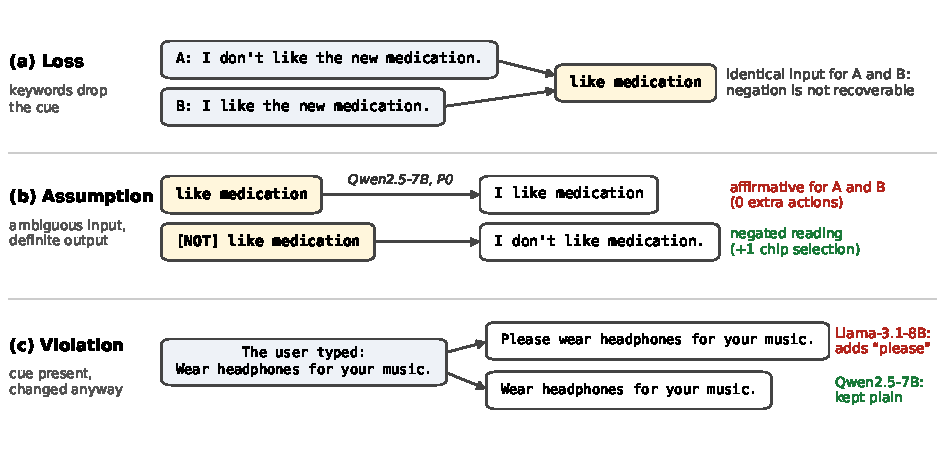
\includegraphics[width=\linewidth]{figs/fig1_running_example}
  \caption{Three sources of meaning change, with real outputs from the main run.
  (a)~Two source messages that differ only in negation map to the same keywords.
  (b)~Given those keywords, the model commits to the affirmative reading for both; one \chip{NOT} chip restores the negated reading.
  (c)~Given the full typed sentence, one model adds ``please'' to a plain directive.
  Selection rule: the first test family of the dimension, prompt P0, Qwen2.5-7B.
  Panel~(c) also shows the first model, in a fixed order, whose output adds ``please''; Qwen2.5-7B kept the sentence plain.
  Script and selected rows: \texttt{figs/make\_fig1.py}, \texttt{figs/fig1\_examples.json}.}
  \Description{Three rows of boxes and arrows. Row a: the sources "I don't like the new medication." and "I like the new medication." both map to the keywords "like medication". Row b: the keywords "like medication" become "I like medication"; "[NOT] like medication" becomes "I don't like medication." Row c: the typed sentence "Wear headphones for your music." becomes "Please wear headphones for your music." with Llama-3.1-8B and stays unchanged with Qwen2.5-7B.}
  \label{fig:example}
\end{figure}

A keyword expander maps an input $x$ to an output sentence $y$.
For a source message $s$, we care about its \emph{commitments}: the values that $s$ makes explicit on six dimensions.
These are polarity, the agent of the main action (speaker, addressee, joint or third party), certainty, time and quantity, speech act (statement, question, request, refusal), and politeness or mitigation.
A commitment is a property of the text, not of the author's private preferences.

We build items as minimal pairs.
A \emph{family} has two source variants that differ on exactly one critical dimension and share the same content words, for example \say{I don't like the new medication} and \say{I like the new medication} (Fig.~\ref{fig:example}a).
Both variants map to the same \emph{bare} keywords (\kw{like medication}), so the bare input cannot tell them apart.
We then vary only what the model receives, the \emph{channel}, and read off the error source from the channel:

\begin{itemize}
\item \textbf{Loss}: the channel does not carry the critical value. For probes this holds by design under the bare channel. For a corpus, we estimate it by checking whether each cue's carrier words survive compression (\S\ref{sec:s1}).
\item \textbf{Violation}: the channel carries the critical cue, through a chip or the full source text, and the output's extracted value differs from the variant's value.
\item \textbf{Assumption}: the channel is ambiguous between the two variants, and the output commits to a definite value anyway. Because both variants receive the identical input, the same output is ``right'' for one and ``wrong'' for the other. We therefore report the commitment rate and its direction, not an accuracy.
\end{itemize}

These are explanatory labels with separate denominators, not mutually exclusive causes.
One case can involve both Loss (compression removed \say{not}) and Assumption (the model then chose \say{like}).
We never sum them into a single breakdown of causes.
An improvement from the bare channel to the full source shows that the output depends on the input channel; it does not reveal the model's internal reasoning.

%% =====================================================================
\section{Method}
%% =====================================================================

\subsection{S1: How often do keywords lose commitments?}
\label{sec:s1}
We use AACText, \num{\RES{s1_n_messages}} fictional messages written by crowd workers who imagined being AAC users (CC BY 4.0)~\cite{vertanen2011imagination}. %CHECK
These are not naturally occurring AAC messages, and we make no claim about any population of AAC users.
A deterministic compressor keeps content words (nouns, proper nouns, main verbs, adjectives, numerals), drops auxiliaries, keeps \say{please}, and truncates to four keywords.
A rule-based detector (spaCy plus lexicons) finds explicit cues for each dimension and checks whether their carrier tokens survive.
Loss is the share of messages with at least one cue whose carrier is absent.
We also compute the minimum number of chips that restores the detected values. Pronoun loss dominates the agent dimension and context can often supply the agent, so our headline excludes agent (Table~\ref{tab:s1}).
We checked the detector against a stratified sample of 400 messages. \pending{independent human check of detector labels} %CHECK

\subsection{S2: Probe families and channels}
The held-out test set has 60 families, 10 per dimension, authored to a fixed specification. %CHECK
Each family records the two sources and their critical values, the shared bare keywords, one noncritical content word (for example \kw{new}), the chips that disambiguate each variant, and the full set of commitments of each variant.
Every variant has at least one chip; the ``unmarked'' variant gets an explicit counter-chip (\chip{YES}, \chip{TELL}, \chip{PLAIN}), so neither variant is resolved for free.
An independent reviewer checked every family against the specification before generation; nine were revised and none dropped. %CHECK
We developed the prompts and codebook on 24 pilot families and 12 development families, then froze them before running the test families. %CHECK
We do not score the ten time and quantity families in this paper: quantity loss is rare in S1, and our time labels are too coarse to score reliably. %CHECK
Table~\ref{tab:families} shows one family per scored dimension.

\begin{table}[t]
  \caption{The first test family of each scored dimension. The bare keywords are shared by both variants.}
  \label{tab:families}
  \small
  \begin{tabular}{@{}lllll@{}}
    \toprule
    Dimension & Variant A & Variant B & Bare input & Chips A / B\\
    \midrule
    Polarity & I don't like the new medication. & I like the new medication. & \kw{like medication} & \chip{NOT} / \chip{YES}\\
    Agent & You left the stove on again. & I left the stove on again. & \kw{leave stove on} & \chip{YOU} / \chip{I}\\
    Certainty & I have a fever again. & I think I have a fever again. & \kw{have fever} & \chip{SURE} / \chip{MAYBE}\\
    Speech act & Can I bring my dog tomorrow? & I'm bringing my dog tomorrow. & \kw{bring dog} & \chip{?} / \chip{TELL}\\
    Politeness & Wear headphones for your music, please. & Wear headphones for your music. & \kw{wear headphones} & \chip{PLEASE} / \chip{PLAIN}\\
    \bottomrule
  \end{tabular}
\end{table}

Each variant is presented through five channels (Table~\ref{tab:channels}).
The \emph{noncrit} channel adds the noncritical word.
It controls for the length and position of the cue: if a chip helps only because the input got longer, a noncritical word should help equally.
Chips are placed before the keywords in a fixed order, and keywords keep their source order.

\begin{table}[t]
  \caption{Channels for variant A of the polarity family, with the action cost under our model. A chip costs one selection. A keyword costs one selection under word prediction, or its characters without it. Typed characters are shown for the full source.}
  \label{tab:channels}
  \small
  \begin{tabular}{@{}lllp{4.7cm}@{}}
    \toprule
    Channel & Model input & Selections (chars) & Role in attribution\\
    \midrule
    bare & \kw{like medication} & 2 (15) & ambiguous: Assumption\\
    noncrit & \kw{like new medication} & 3 (19) & length control, still ambiguous\\
    chip1 & \kw{[NOT] like medication} & 3 (15 + 1 chip) & critical cue given: Violation\\
    chipall & \kw{[NOT] [TELL] [I] like medication} & 5 (15 + 3 chips) & all commitments given: Violation\\
    full & \kw{The user typed: I don't like\ldots} & -- (32) & oracle: errors are Violation only\\
    \bottomrule
  \end{tabular}
\end{table}

\paragraph{Chips and cost.}
The chip vocabulary covers polarity (\chip{NOT}, \chip{YES}), speech act (\chip{?}, \chip{ASK}, \chip{REFUSE}, \chip{TELL}), certainty (\chip{MAYBE}, \chip{SURE}, \chip{MUST}, \chip{WANT}), agent (\chip{I}, \chip{YOU}, \chip{WE}, \chip{THEY}), time (\chip{PAST}, \chip{NOW}, \chip{LATER}), exact numbers, and politeness (\chip{PLEASE}, \chip{PLAIN}).
Every prompt includes the same legend, so all channels receive the same instructions.
We count one action per chip, one per keyword under word prediction (or its characters without prediction), and one per suggestion picked from a list.
This is a deliberately simple proxy.
Reading and checking suggestions costs real time~\cite{cai2024speakfaster,waller2025typetalk}, and we do not measure effort, fatigue, or speed.

\subsection{Prompts and models}
All prompts describe the task as the sentence-composition feature of an AAC app.
\textbf{P0} asks for \say{the single sentence they are trying to say} and decodes greedily.
\textbf{S3} uses P0 with three samples at temperature 0.7, a natural multi-suggestion baseline.
\textbf{P2} asks for \say{3 different suggestions that cover the different things the user might mean} as a JSON list and decodes greedily.
For S3 and P2, each suggestion is scored on its own.
We piloted a preservation prompt; it changed critical match by $-3$ to $+7$ points across channels on unvalidated pilot labels, at our pre-set kill line, so we dropped it before the main run to fund validation. %CHECK
We test three open models run locally with 4-bit quantization (Qwen2.5-7B-Instruct, Llama-3.1-8B-Instruct, Gemma-3-4B-it; Q4\_K\_M GGUF via llama.cpp) and one API model (gpt-6.1-terra).
Local models reflect on-device deployment; we do not measure latency or privacy.
Prompts, seeds, model hashes and every raw output are logged.

\subsection{Label extraction: a judge that cannot see the answer}
Judges never see the source message, the model, the prompt, or the channel.
They see one output sentence and answer extraction questions with fixed options.
The critical question asks what value the output expresses for the family's dimension, with \say{unclear/mixed} always available.
The general questions cover polarity, speech act, agent, certainty and politeness.
A second pass shows the visible input and asks whether the output adds a fact, reason, person, place or time that the input does not contain.
Loss, Violation and Assumption are then computed deterministically from the extracted values, the item specification and the channel.
Identical output texts are judged once, whatever model or condition produced them.

The judge is gpt-6.1-sol, a different model from the GPT model under test.
Two prompt variants differ in wording, option order and item order; if they disagree, a cross-family arbiter (a Claude model) decides.
Because judges can favor outputs from their own model family~\cite{panickssery2024selfpreference}, we report the GPT generation arm's validation separately. %CHECK
The codebook fixes edge cases before scoring.
\say{Can you\ldots?} is a request without politeness, \say{Can I\ldots?} is a question, and \say{I want X} has the speaker as agent.
For certainty, an emphatic output matches a plain assertion and is logged as an added stance.

\subsection{Human validation}
Two anonymous annotators, neither an author, labeled \num{\RES{gold_n}} held-out outputs, using the same options and the same output-only view as the judge: they saw only the output sentence, plus the visible input when coding added content, with no model, condition or source shown. %CHECK
The outputs were drawn with known inclusion probabilities, stratified by dimension, model and channel. %CHECK
Coders also labeled \num{\RES{challenge_n}} authored challenge sentences: semantic mutations, such as a dropped negation or a swapped agent, and meaning-preserving paraphrases. %CHECK
We report Krippendorff's $\alpha$ between coders before adjudication, and Cohen's $\kappa$, sensitivity and specificity of the final judge pipeline against adjudicated labels. %CHECK
We use a dimension's judge labels only if its $\kappa \geq 0.6$; otherwise we report that dimension from human labels alone. %CHECK

\subsection{Statistics}
Outputs within a family are not independent: two variants share one bare request, and three suggestions share one set.
We therefore resample whole families (\num{\RES{n_families_scored}} scored families), keeping all variants, channels, prompts and models of each sampled family together, and recompute every estimate and paired contrast in each of 2,000 replicates. %CHECK
We report 95\% percentile intervals with equal family weights~\cite{saravanan2020hierarchical}.
Corpus rates in S1 carry Wilson intervals over messages.

%% =====================================================================
\section{Results}
%% =====================================================================
%% Every number-dependent sentence below is written for the direction seen in the pilot.
%% If a main-run estimate reverses direction, rewrite the sentence; do not just swap the number.

\subsection{Loss: keywords drop commitments in most messages}
\begin{table}[t]
  \caption{S1 on AACText (\num{\RES{s1_n_messages}} messages). Percentage of messages; 95\% Wilson intervals in brackets. Detector-based estimates of cue-token loss, not semantic judgments.}
  \label{tab:s1}
  \small
  \begin{tabular}{@{}lr@{}}
    \toprule
    Measure (POS-cap4 compressor) & \% of messages\\
    \midrule
    Loses $\geq$1 detected cue, any dimension & \num{\RES{s1_loss_any}} \ci{s1_loss_any}\\
    \quad excluding agent (pronoun) loss & \num{\RES{s1_loss_excl_agent}} \ci{s1_loss_excl_agent}\\
    \quad excluding agent and time & \num{\RES{s1_loss_excl_agent_time}}\\
    Loses a negation cue & \num{\RES{s1_loss_polarity}}\\
    Loses a speech-act cue & \num{\RES{s1_loss_speech_act}}\\
    Keywords collide with a differently labeled message & \num{\RES{s1_collision}}\\
    All detected values restorable with $\leq$2 chips & \num{\RES{s1_restore_two}}\\
    Loss not expressible in the chip vocabulary & \num{\RES{s1_inexpressible}}\\
    \bottomrule
  \end{tabular}
\end{table}
Content-word keywords lose at least one explicit cue in \num{\RES{s1_loss_excl_agent}}\% of AACText messages, even when we ignore pronouns (Table~\ref{tab:s1}). %CHECK
Speech act is the most frequently lost dimension after agent and time: question and request forms are carried by function words and word order that the compressor removes. %CHECK
Negation is rarer but is always lost when present, because the compressor removes \say{not}. %CHECK
In \num{\RES{s1_collision}}\% of messages, the keywords are identical to those of another message with a different commitment, so even a perfect expander could not recover both. %CHECK
Two chips or fewer would restore all detected values in \num{\RES{s1_restore_two}}\% of messages. %CHECK
This counts category values, not phrasing or negation scope. Loss is common, and cheap to mark in principle; what models do with the gap is a separate question.

\subsection{Assumption: the unmarked reading is free}
\label{sec:res-default}
Under the bare channel, \num{\RES{bare_affirm_rate}}\% \ci{bare_affirm_rate} of definite polarity outputs were affirmative (\num{\RES{bare_affirm_n}}/\num{\RES{bare_affirm_den}}), across all four models and all prompts. %CHECK
The spanning prompt P2, which explicitly asks the model to cover different meanings, offered a negated suggestion in \num{\RES{bare_neg_offered_p2}}\% of polarity sets. %CHECK
Defaults appear on other dimensions as well, though they are less extreme.
Bare outputs named the speaker as agent in \num{\RES{bare_speaker_rate}}\% of agent-family outputs, and used a plain assertion in \num{\RES{bare_plain_cert_rate}}\% of certainty-family outputs. %CHECK
They added \say{please} or a softener in \num{\RES{bare_please_added}}\% of outputs where the input had neither. %CHECK

Adding the noncritical word changed the aggregate critical-match rate by \num{\RES{noncrit_vs_bare}} points \ci{noncrit_vs_bare}. %CHECK
It did change individual outputs (\num{\RES{noncrit_rows_differ}}\% of aligned rows), so we claim only that a longer input does not by itself move the aggregate default. %CHECK

Figure~\ref{fig:cost} turns these rates into a cost.
For a person who means the affirmative, the bare keywords already produce the intended polarity, at zero extra actions.
For a person who means the negation, the bare keywords produce the opposite, and the intended meaning becomes available only after an extra selection. %CHECK
At the bare channel, the paired fidelity gap between the two directions was \num{\RES{action_gap_polarity}} points \ci{action_gap_polarity}. %CHECK
The minimum tested cost to reach 80\% fidelity was \num{\RES{min_actions_aff}} extra actions for affirmative variants and \num{\RES{min_actions_neg}} for negated ones. %CHECK
The asymmetry is not a measurement artifact of our choice of base rate: the same bare input serves both variants, so any model that always picks one reading charges the other reading's speaker for every correction.
Who pays is decided by the default, not by the person.

\begin{figure}[t]
  \centering
  \IfFileExists{figs/fig2_action_cost.pdf}{%
    \includegraphics[width=\linewidth]{figs/fig2_action_cost}%
  }{%
    \fbox{\parbox[c][4.5cm][c]{0.9\linewidth}{\centering\small
      PLACEHOLDER for \texttt{figs/fig2\_action\_cost.pdf} (generated by the analysis).\\[2pt]
      Panels by dimension. x: extra input actions beyond the keywords (bare $=0$, chip1 $=1$, chipall $=$ number of chips).\\
      y: critical-value fidelity with family-bootstrap 95\% intervals.\\
      One line per direction (unmarked vs.\ marked variant), pooled over models; thresholds that are never reached are marked.}}%
  }
  \caption{Fidelity against input actions, separately for each direction of each minimal pair. Under the bare channel the unmarked reading starts high and the marked reading starts low. One chip closes most of the gap. %CHECK
  Intervals come from resampling families.}
  \Description{Line plots of fidelity against the number of extra input actions for each commitment dimension, with one line for the unmarked variant and one for the marked variant.}
  \label{fig:cost}
\end{figure}

\subsection{Violation: cues mostly survive, explicit politeness choices do not}
With one chip, polarity was preserved in \num{\RES{chip1_match}}\% \ci{chip1_match} of outputs. %CHECK
Across scored dimensions, one chip reached \num{\RES{chip1_match_all}}\% critical match, against \num{\RES{full_match_all}}\% when the model saw the full source (difference \num{\RES{chip1_vs_full}} points \ci{chip1_vs_full}; Table~\ref{tab:match}). %CHECK
In other words, a single selection recovers most of what the typed sentence provides on the tested dimension. %CHECK

The full channel is the most instructive, because there the model sees exactly what the person typed.
Models still changed it.
For plain directives presented in full, \num{\RES{full_politeness_added}}\% \ci{full_politeness_added} of outputs added \say{please} or a softener (\num{\RES{full_politeness_added_n}}/\num{\RES{full_politeness_added_den}}). %CHECK
Fig.~\ref{fig:example}c shows one: \say{Wear headphones for your music.} became \say{Please wear headphones for your music.}
Overall, \num{\RES{full_stance_changed}}\% of full-channel outputs changed at least one explicit value on a general dimension. %CHECK
Violations concentrated in speech act and politeness, not in polarity or agent. %CHECK
These changes look minor, and that is the point: an assistant tuned to be courteous treats a deliberately plain request as a draft to improve~\cite{chalfoun2025please,agarwal2025homogenize}.

\begin{table}[t]
  \caption{Critical-value match (\%) by dimension and channel, prompt P0, pooled over four models. For bare and noncrit the input is ambiguous, so match is at most the share of the more frequent variant and is not an accuracy. %CHECK
  }
  \label{tab:match}
  \small
  \begin{tabular}{@{}lrrrrr@{}}
    \toprule
    Dimension & bare & noncrit & chip1 & chipall & full\\
    \midrule
    Polarity   & \num{\RES{match_pol_bare}} & \num{\RES{match_pol_noncrit}} & \num{\RES{match_pol_chip1}} & \num{\RES{match_pol_chipall}} & \num{\RES{match_pol_full}}\\
    Agent      & \num{\RES{match_agt_bare}} & \num{\RES{match_agt_noncrit}} & \num{\RES{match_agt_chip1}} & \num{\RES{match_agt_chipall}} & \num{\RES{match_agt_full}}\\
    Certainty  & \num{\RES{match_cer_bare}} & \num{\RES{match_cer_noncrit}} & \num{\RES{match_cer_chip1}} & \num{\RES{match_cer_chipall}} & \num{\RES{match_cer_full}}\\
    Speech act & \num{\RES{match_act_bare}} & \num{\RES{match_act_noncrit}} & \num{\RES{match_act_chip1}} & \num{\RES{match_act_chipall}} & \num{\RES{match_act_full}}\\
    Politeness & \num{\RES{match_pz_bare}}  & \num{\RES{match_pz_noncrit}}  & \num{\RES{match_pz_chip1}}  & \num{\RES{match_pz_chipall}}  & \num{\RES{match_pz_full}}\\
    \bottomrule
  \end{tabular}
\end{table}

\subsection{Cue interaction: one more chip can undo a choice}
\label{sec:res-interaction}
Giving a model more commitments does not simply add up.
In the pilot, \chip{PLAIN} alone kept requests plain, but \chip{ASK} \chip{YOU} \chip{PLAIN} led one model to add \say{please}. %CHECK
On the first held-out politeness family, Gemma-3-4B turned \kw{[ASK] [YOU] [PLAIN] wear headphones} into \say{Could you please tell me if you are wearing headphones?}, which adds a softener and also changes the request into a question about the listener's state.
We tested this effect directly (Experiment~B).
Holding \chip{PLAIN} or \chip{PLEASE} fixed on held-out politeness families, we crossed the presence of \chip{ASK} and \chip{YOU}, and added a control with inert bracketed tags of matched length. %CHECK
Adding \chip{ASK} and \chip{YOU} lowered plainness preservation by \num{\RES{interaction_drop}} points \ci{interaction_drop}, against \num{\RES{interaction_padding_drop}} points for the padding control, in \num{\RES{interaction_families}} families. %CHECK
\pending{state which models show the effect; the pilot effect in Qwen disappeared once labels followed the codebook (see \S\ref{sec:res-oracle}); report a model-specific counterexample if only one model shows it} %CHECK
Re-encoding the same commitments as transparent aliases or as short natural-language fields changed critical match by \num{\RES{encoding_alias_delta}} and \num{\RES{encoding_nl_delta}} points, respectively. %CHECK
In a factorial test that crossed polarity and actor cues on eight new families (Experiment~C), adding the second cue lowered accuracy on the first by \num{\RES{factorial_protected_drop}} points \ci{factorial_protected_drop}. %CHECK
Lower joint accuracy than either single cue is expected arithmetically; we report the drop on the already specified dimension, which is the quantity that matters to the person.

\subsection{Suggestion sets: they span politeness, not polarity}
Asking for three suggestions that cover different meanings (P2) covered both readings of a family in \num{\RES{coverage_p2}}\% \ci{coverage_p2} of bare sets, against \num{\RES{coverage_s3}}\% \ci{coverage_s3} for three sampled outputs (S3). %CHECK
The gain came mostly from politeness (\num{\RES{coverage_p2_pz}}\% vs.\ \num{\RES{coverage_s3_pz}}\%). %CHECK
For polarity, neither P2 nor S3 covered the negated reading (\num{\RES{coverage_p2_pol}}\% vs.\ \num{\RES{coverage_s3_pol}}\%). %CHECK
P2 suggestions added unlicensed content more often than S3 samples (\num{\RES{p2_additions}}\% vs.\ \num{\RES{s3_additions}}\%). %CHECK
Asking a model to diversify does not make it offer the reading that it never chooses by default.

\subsection{Is the oracle trustworthy?}
\label{sec:res-oracle}
The two human coders agreed at $\alpha=\num{\RES{human_alpha}}$ \ci{human_alpha} before adjudication. %CHECK
The final judge pipeline agreed with adjudicated labels at $\kappa=\num{\RES{judge_kappa}}$ \ci{judge_kappa} on the critical dimension; the lowest per-dimension $\kappa$ was \num{\RES{judge_kappa_min}}. %CHECK
For Violation events, the judge's sensitivity was \num{\RES{judge_sens_violation}}\% and its specificity \num{\RES{judge_spec_violation}}\%; it labeled \num{\RES{challenge_acc}}\% of challenge sentences correctly. %CHECK
Validation changed conclusions, not just error bars.
Our pilot's deterministic labeler counted \say{Can you\ldots?} as a softened request, which made one model appear to lose plainness whenever \chip{ASK} was added.
Under the codebook rule, the same outputs are plain, and that apparent effect disappeared.
Across headline contrasts, \num{\RES{stale_label_flips}} changed by ten points or more between unvalidated and validated labels. %CHECK
\pending{if the validation gate fails for a dimension, say here which results rest on human labels only}

%% =====================================================================
\section{Discussion}
%% =====================================================================

\paragraph{Defaults are a policy choice.}
An expander that always picks the affirmative, the plain assertion, or the polite request has a policy, whether or not anyone wrote it down.
The policy decides whose meaning arrives at zero cost and whose meaning needs an extra action.
For a person who often refuses, negates, or speaks plainly, the system charges that person each time.
How often any individual means the non-default reading, only they can say; but the designer sets the charge, and should do so on purpose and in the open.

\paragraph{Make non-default meanings cheap and visible.}
Commitment chips worked as an input channel: one selection recovered most of the full-source fidelity on the tested dimension. %CHECK
Chips need not be new widgets; intent buttons and stance tags already exist~\cite{valencia2024compa,mao2025designprobes,xiang2025socializechat}.
Our results suggest three refinements.
First, place \chip{NOT}, \chip{?} and \chip{MAYBE} where they cost one selection, since these are the cues that the defaults override. %CHECK
Second, test combinations of chips, not only single chips, because one chip can undo another. %CHECK
Third, show the person which commitments the output makes, for example by highlighting \say{please} or a dropped hedge, so that a change is visible before the sentence is spoken.

\paragraph{Suggestion sets should span readings, not wordings.}
Where the input is ambiguous on a dimension that matters, such as polarity, a set should contain each reading, including the one the model would not choose on its own.
Templates or explicit reading enumeration can guarantee this where prompting does not~\cite{saparina2026reasoningintent}. %CHECK

\paragraph{Never soften a plain directive the person typed.}
When the input already contains a complete sentence, the expander has nothing to expand.
Adding \say{please} to \say{Wear headphones for your music} is a small edit, but it is the system speaking in the person's place.
Some people may want an optional politeness assistant; that should be a setting they turn on, not a behavior they must notice and undo.

\paragraph{Limitations.}
We ran no study with AAC users, so we cannot speak to agency, effort, fatigue, or whether anyone wants a given output.
AACText is fictional, crowd-written text, and our probes are constructed; neither shows what AAC users actually mean.
Our cost model counts selections only and leaves out reading and checking suggestions, which can be substantial~\cite{waller2025typetalk}.
Commitments are text-explicit categories: a chip restores \chip{NOT} but not its scope, and we did not score time and quantity.
The judge is an LLM; we validated it against human labels on a limited sample, and dimensions below our agreement threshold rest on human labels alone. %CHECK
We tested four models, three of them small quantized models, with fixed prompts and no conversation context; larger models, context or personalization may shift the defaults.
Ten families per dimension support estimates for these models and items, not population rates.
No autistic advisers or community reviewers took part; future work should involve autistic AAC users and advisers directly.

\paragraph{Autistic-informed, not essentialist.}
Our definitions of an added commitment, especially for directness, hedging and politeness, rest on the autism and participatory-research literature, not on community review (\S\ref{sec:ethics}).
They do not make our probes autistic speech, and they do not support any claim that autistic people write in a particular way.
We treat directness as one legitimate choice among others, to be kept when the person makes it, not as a trait to detect or correct.

%% =====================================================================
\section{Ethics and Positionality}
\label{sec:ethics}
%% =====================================================================
This study collected no data from AAC users and no personal preference data.
AACText is public under CC BY 4.0 and contains fictional messages~\cite{vertanen2011imagination}.
Two anonymous annotators, neither an author, labeled model outputs under a fixed codebook, blinded to model, condition and source.
As independent researchers we did not obtain an institutional review determination; annotators labelled machine-generated sentences, were reimbursed, and no personal data were collected beyond an annotator ID. % AUTHOR-CONFIRM: ethics sentence
\pending{Author positionality: state, as each author chooses, relevant lived experience (for example being autistic or using AAC) and disciplinary background, and how it shaped the work.}

\paragraph{Research measures without advisers.}
No autistic advisers or community reviewers took part in this study.
Instead, we addressed the problems of an earlier version of this study through expert literature and literature reviews.
A critical review of that version retired its synthetic autistic-vs-neurotypical comparison.
The design draws on autism and participatory-research guidance, including AASPIRE~\cite{nicolaidis2019aaspire}, the double-empathy problem~\cite{milton2012double}, and cautions about heterogeneity among autistic AAC users~\cite{zisk2019aac,frisch2025autistic}.
We assume no ``autistic style'', and we limit claims to commitments explicit in the text.
Reviews of advisory practice in autism research~\cite{jansevanrensburg2026advisory} describe what such direct involvement would add.

\paragraph{Release.}
\pending{Repository URL with probe families, codebook, prompts, raw outputs, judge prompts and labels, and analysis code.}

\begin{acknowledgments}
\pending{Acknowledgments, including the two annotators if they wish to be thanked.}
\end{acknowledgments}

%% CEUR mandatory section. Must be truthful and follow https://ceur-ws.org/GenAI/Policy.html
%% and the taxonomy at ceur-ws.org/genai-tax.html. Note: in this study LLMs are also the OBJECT of
%% study (models under test) and research instruments (judge, arbiter). Keep that separate from
%% writing assistance. CEUR does not allow GenAI-generated paragraphs or sections: the authors
%% must write the final text themselves.
\section*{Declaration on Generative AI}
\pending{Replace with an accurate declaration. List every GenAI tool and service used and what each did, categorized with the CEUR GenAI Usage Taxonomy (for example literature search, code generation, drafting, figure scripting). Then state: ``After using these tools/services, the authors reviewed and edited the content as needed and take full responsibility for the publication's content.'' Describe the models under test and the LLM judge as research instruments in the Method section, not here.}

\bibliography{refs}

\end{document}
